\documentclass[12pt, legalpaper]{exam}
\usepackage[utf8]{inputenc}
\usepackage[english]{babel}
\usepackage[margin=.8in]{geometry}
\usepackage{amsmath,amssymb}
\usepackage{multicol}
\usepackage{graphicx}
\usepackage{tikz}
\usepackage{lastpage}
\usepackage{tabularx}
\usepackage{hyperref}
\usepackage{tcolorbox}
\newcommand{\course}{Introduction to Optimization}
\newcommand{\term}{Fall 2024}
\newcommand{\examnum}{Report of Programming Task 1}


\begin{document}
\noindent \examnum \, of the  course ''\course'' - \term


\noindent
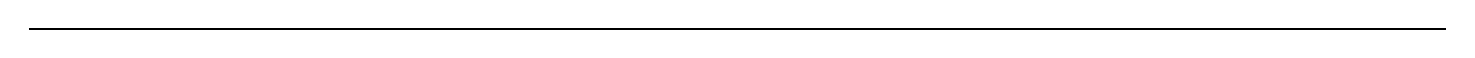
\begin{tikzpicture}
\draw[thick] (0,0) -- (18,0);
\end{tikzpicture}




\vspace{12pt}
\begin{center}
    \textbf{Report 1}
\end{center}
% \noindent \textbf{Requirements}

\vspace{12pt}

\noindent  \textbf{Team information.}

\begin{itemize}
    \item Team leader: Nikita Tsukanov 
    \item Team member 1: Dmitriy Tetkin
    \item Team member 2: Mikhail Trifonov
    \item Team member 3: Ilsaf Abdulkhakov
\end{itemize}
\vspace{12pt}
\noindent  \textbf{Team participation}
\begin{itemize}
    \item Nikita Tsukanov - 5/5 grade
    \item Dmitriy Tetkin - 5/5 grade
    \item Mikhail Trifonov - 5/5 grade
    \item Ilsaf Abdulkhakov - 5/5 grade
\end{itemize}
\vspace{12pt}

\noindent     \textbf{Link to the product.}
\begin{itemize}
    \item The product is available: https://github.com/Optimization-Innopolis/task1
\end{itemize}

\vspace{12pt}

\noindent  \textbf{Programming language.}
\begin{itemize}
    \item Programming language: Python
\end{itemize}

\vspace{12pt}

\noindent  \textbf{Linear programming problem.}
\begin{itemize}
\item Maximization or Minimization? - Maximization
\vspace{10pt}
    \item  LLP:
    A company produces two products, Product 1 and Product 2. The profit from selling each unit of Product 1 is \$3, while the profit from selling each unit of Product 2 is \$2. The company wants to maximize its total profit.

Each unit of Product 1 requires 2 units of Resource A and each unit of Product 2 requires 1 unit of Resource A. The total available units of Resource A are 10. The company can produce a maximum of 8 units in total of both products combined. The production of Product 1 cannot exceed 4 units.

Product 1 denoted as \( x_1 \) and Product 2 denoted as \( x_2 \)
    \item Objective function:
    \[
  \text{Maximize } z = 3x_1 + 2x_2
  \]
    \vspace{10pt}    
    \item Constraint functions:
    \[
  2x_1 + 1x_2 \leq 10 \quad \text{(Resource A constraint)}
  \]
  \[
  x_1 + x_2 \leq 8 \quad \text{(Total production constraint)}
  \]
  \[
  x_1 \leq 4 \quad \text{(Maximum production of Product 1)}
  \]
  \[
  x_1, x_2 \geq 0 \quad \text{(Non-negativity constraints)}
  \]
\end{itemize}


\subsection*{Result}
The input contains:
\begin{itemize}
    \item A vector of coefficients of objective function: $\mathbf{C} = [3, 2]$
    \item A matrix of coefficients of constraint function:
    \[
    \mathbf{A} =
    \begin{bmatrix}
    2 & 1 \\
    1 & 1 \\
    1 & 0
    \end{bmatrix}
    \]
    \item A vector of right-hand side numbers: $\mathbf{b} = [10, 8, 4]$
    \item Approximation accuracy: $\epsilon = 0.001$
\end{itemize}

\noindent  \textbf{Output}
\begin{itemize}
    \item Solver State: solved
    \item A vector of decision variables: $\mathbf{X^*} = [2.0, 6.0]$
    \item Maximum value of the objective function: $z = 18.0$
\end{itemize}

\vspace{1cm}

\subsection*{Test1}
The input contains:
\begin{itemize}
    \item A vector of coefficients of objective function: $\mathbf{C} = [5, 4]$
    \item A matrix of coefficients of constraint function:
    \[
    \mathbf{A} =
    \begin{bmatrix}
    1 & 2 \\
    3 & 2
    \end{bmatrix}
    \]
    \item A vector of right-hand side numbers: $\mathbf{b} = [6, 12]$
    \item Approximation accuracy: $\epsilon = 0.001$
\end{itemize}

\noindent  \textbf{Output}
\begin{itemize}
    \item Solver State: solved
    \item A vector of decision variables: $\mathbf{X^*} = [3.0, 1.5]$
    \item Maximum value of the objective function: $z = 21.0$
\end{itemize}

\vspace{1cm}

\subsection*{Test2}
The input contains:
\begin{itemize}
    \item A vector of coefficients of objective function: $\mathbf{C} = [6, 8]$
    \item A matrix of coefficients of constraint function:
    \[
    \mathbf{A} =
    \begin{bmatrix}
    1 & 1 \\
    5 & 4
    \end{bmatrix}
    \]
    \item A vector of right-hand side numbers: $\mathbf{b} = [10, 40]$
    \item Approximation accuracy: $\epsilon = 0.001$
\end{itemize}

\noindent  \textbf{Output}
\begin{itemize}
    \item Solver State: solved
    \item A vector of decision variables: $\mathbf{X^*} = [0.0, 10.0]$
    \item Maximum value of the objective function: $z = 80.0$
\end{itemize}

\vspace{1cm}

\subsection*{Test3}
The input contains:
\begin{itemize}
    \item A vector of coefficients of objective function: $\mathbf{C} = [4, 3]$
    \item A matrix of coefficients of constraint function:
    \[
    \mathbf{A} =
    \begin{bmatrix}
    -1 & 1
    \end{bmatrix}
    \]
    \item A vector of right-hand side numbers: $\mathbf{b} = [2]$
    \item Approximation accuracy: $\epsilon = 0.001$
\end{itemize}

\noindent  \textbf{Output}
\begin{itemize}
    \item Solver State: unbounded
\end{itemize}

\vspace{1cm}


\subsection*{Test4}
The input contains:
\begin{itemize}
    \item A vector of coefficients of objective function: $\mathbf{C} = [10, 6]$
    \item A matrix of coefficients of constraint function:
    \[
    \mathbf{A} =
    \begin{bmatrix}
    1 & 1 \\
    2 & 1 \\
    1 & 2
    \end{bmatrix}
    \]
    \item A vector of right-hand side numbers: $\mathbf{b} = [100, 150, 120]$
    \item Approximation accuracy: $\epsilon = 0.001$
\end{itemize}

\noindent  \textbf{Output}
\begin{itemize}
    \item Solver State: solved
    \item A vector of decision variables: $\mathbf{X^*} = [60.0, 30.0]$
    \item Maximum value of the objective function: $z = 780.0$
\end{itemize}

\vspace{1cm}

\subsection*{Test5}
The input contains:
\begin{itemize}
    \item A vector of coefficients of objective function: $\mathbf{C} = [2, 5]$
    \item A matrix of coefficients of constraint function:
    \[
    \mathbf{A} =
    \begin{bmatrix}
    1 & 2 \\
    2 & 1
    \end{bmatrix}
    \]
    \item A vector of right-hand side numbers: $\mathbf{b} = [20, 18]$
    \item Approximation accuracy: $\epsilon = 0.001$
\end{itemize}

\noindent  \textbf{Output}
\begin{itemize}
    \item Solver State: solved
    \item A vector of decision variables: $\mathbf{X^*} = [0.0, 10.0]$
    \item Maximum value of the objective function: $z = 50.0$
\end{itemize}

\vspace{1cm}

\noindent
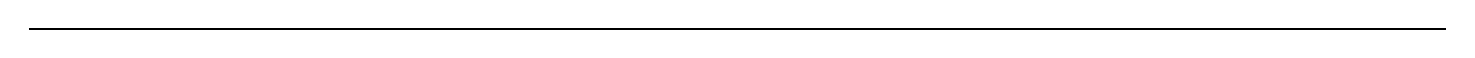
\begin{tikzpicture}
\draw[thick] (0,0) -- (18,0);
\end{tikzpicture}




\vspace{24pt}
\noindent     \textbf{Code}

\begin{verbatim}
import numpy as np


def simplex_solver(C, A, b, eps=1e-9):
    C = np.array(C)

    print("Optimization Problem:")
    objective_type = "max" if all(c <= 0 for c in C) else "min"
    obj_func = " + ".join(f"{C[i]} * x{i + 1}" for i in range(len(C)))
    print(f"{objective_type} z = {obj_func}")

    print("Subject to the constraints:")
    for i in range(len(A)):
        constraints = " + ".join(f"{A[i][j]} * x{j + 1}" for j in range(len(A[i])))
        print(f"{constraints} <= {b[i]}")

    num_vars = len(C)
    num_constraints = len(A)

    tableau = np.zeros((num_constraints + 1, num_vars + num_constraints + 1))

    tableau[:num_constraints, :num_vars] = A
    tableau[:num_constraints, num_vars:num_vars + num_constraints] = np.eye(num_constraints)
    tableau[:num_constraints, -1] = b
    tableau[-1, :num_vars] = -C

    while True:
        entering_var_index = np.argmin(tableau[-1, :-1])
        entering_var_coeff = tableau[-1, entering_var_index]

        if entering_var_coeff >= -eps:
            break

        ratios = []
        for i in range(num_constraints):
            if tableau[i, entering_var_index] > eps:
                ratios.append(tableau[i, -1] / tableau[i, entering_var_index])
            else:
                ratios.append(float('inf'))

        leaving_var_index = np.argmin(ratios)

        if ratios[leaving_var_index] == float('inf'):
            return {"solver_state": "unbounded", "x_star": None, "z": None}

        pivot_value = tableau[leaving_var_index, entering_var_index]
        tableau[leaving_var_index] /= pivot_value

        for i in range(num_constraints + 1):
            if i != leaving_var_index:
                tableau[i] -= tableau[i, entering_var_index] * tableau[leaving_var_index]

    solution = np.zeros(num_vars)
    for i in range(num_vars):
        col = tableau[:, i]
        if sum(col == 1) == 1 and sum(col == 0) == num_constraints:
            row = np.where(col == 1)[0][0]
            solution[i] = tableau[row, -1]

    optimal_value = tableau[-1, -1]

    return {"solver_state": "solved", "x_star": solution, "z": optimal_value}


def run_tests():
    tests = [
        # Special Case: Degeneracy
        {
            "name": "Degenerate Case",
            "C": [5, 4],
            "A": [[1, 2], [3, 2]],
            "b": [6, 12],
        },
        # Special Case: Alternative Optima (Multiple optimal solutions)
        {
            "name": "Alternative Optima",
            "C": [6, 8],
            "A": [[1, 1], [5, 4]],
            "b": [10, 40],
        },
        # Special Case: Unbounded Solution
        {
            "name": "Unbounded Solution",
            "C": [4, 3],
            "A": [[-1, 1]],
            "b": [2],
        },
        # Standard Maximization LPP 1
        {
            "name": "Maximization LPP 1",
            "C": [3, 2],
            "A": [[2, 1], [1, 1], [1, 0]],
            "b": [10, 8, 4],
            "eps": 1e-9  # Default epsilon
        },
        # Standard Maximization LPP 2 with custom epsilon
        {
            "name": "Maximization LPP 2",
            "C": [10, 6],
            "A": [[1, 1], [2, 1], [1, 2]],
            "b": [100, 150, 120],
            "eps": 1e-6  # Custom epsilon for this test case
        },
        # Standard Maximization LPP 3 with custom epsilon
        {
            "name": "Maximization LPP 3",
            "C": [2, 5],
            "A": [[1, 2], [2, 1]],
            "b": [20, 18],
            "eps": 1e-9  # Default epsilon
        },
        # Standard Maximization LPP 4
        {
            "name": "Maximization LPP 4",
            "C": [8, 6],
            "A": [[2, 1], [1, 3]],
            "b": [16, 15],
            "eps": 1e-9  # Default epsilon
        }
    ]

    for test in tests:
        eps = test.get('eps', 1e-9)
        print("Test:", test['name'])
        result = simplex_solver(test['C'], test['A'], test['b'], eps)
        print("\nResult:")
        print("Solver State:", result['solver_state'])
        if result['solver_state'] == "solved":
            print("Optimal Decision Variables (x*):", result['x_star'])
            print("Optimal Value (z):", result['z'])
        print()


# Uncomment to run our tests
# run_tests()

\end{verbatim}

\end{document}